\chapter{Implementación} % Main chapter title
\label{Chapter5}
\lhead{Capítulo 5. \emph{Implementación}}
\setstretch{1.1} % Line spacing of 1.1
El presente capítulo describe los detalles de la implementación de los requerimientos explicados en el capítulo \ref{Chapter4}. %En la primera parte
Se desarrollará el sistema completo localmente en una computadora de uso común. Para explicar el tratamiento que recibe un acta en la aplicación, se usan diagramas de actividad detalladas y se realizan pruebas sobre cada etapa antes de proceder con la siguiente.

%En la segunda parte se describen las modificaciones necesarias para que dicho sistema pueda ser desplegado en un clúster de Kubernetes junto con las pruebas correspondientes en el ambiente de desarrollo microk8s.
\section{Implementación Local}
La implementación local del proyecto fue realizada en una Notebook MSI PL62 7RC, el sistema operativo empleado fue Ubuntu 16.04 LTS. Las características de la máquina se detallan en la figura \ref{fig:msi_c5}
\begin{figure}
    \center{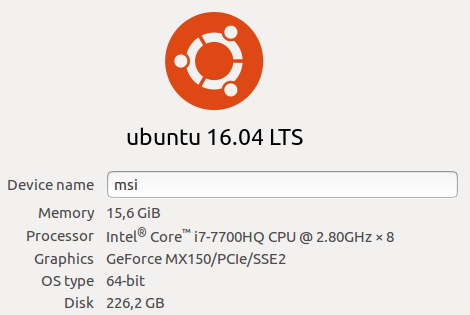
\includegraphics[width=0.6\linewidth]{Figures/Selection_189.png}}
    \caption{Características técnicas de la computadora de desarrollo.}
    \label{fig:msi_c5}
\end{figure}
\subsection{Configuración de Hyperledger Fabric}
Antes de iniciar la implementación de la aplicación en sí, es necesario configurar una red y un Blockchain con Hyperledger Fabric. Esta sección describe los pasos necesarios para cumplir con dicho objetivo.
\begin{enumerate}
    \item \textbf{Generación de certificados con la herramienta cryptogen:} Como descrito en la sección \ref{sec:identidad_de_peers}, cada integrante de la red establece su identidad a través de un certificado X.509. Hyperledger Fabric provee una herramienta llamada cryptogen que genera un conjunto de certificados y claves, así una red puede ser iniciada fácilmente con todo el material criptográfico necesario.
    
    Cryptogen lee la arquitectura deseada de la red desde un archivo con formato \textit{yaml} y genera los certificados acorde a dicho archivo. Por ende, el primer paso para la configuración de la red fue expresar su topología deseada de la siguiente forma:
    \inputminted[linenos, bgcolor=mygray]{yaml}{Listings/crypto-config.yaml}
    Las primeras cinco líneas definen una organización para el servicio que ordena las transacciones, con su nombre y dominio. Se eligió pi.elisabeth.com, donde pi es la abreviación de proyecto integrador. El dominio del cualquier \textit{peer} está compuesto por su \textit{hostname} y el dominio de la organización, por lo cual se accede como orderer.pi.elisabeth.com. Como se va a emplear el servicio \textit{solo}, se emplea a un solo host para dicha tarea.

    En la segunda sección, línea 7 a 30, se definen las organizaciones de los \textit{peers}. Para eso, se eligieron 3 facultades de la UNC y se definieron 2 \textit{peers} por cada facultad, indicados por las líneas 12, 20 y 28. La propiedad \textit{Users} está pensada para definir de forma anticipada la cantidad de usuarios que van a utilizar el Blockchain. En el caso del prototipo a desarrollar, este aspecto se va a definir de forma dinámica, por lo cual el archivo indica 1 usuario de modo que se cree solo un usuario administrador.
    
    Una vez que se pudo establecer una organización lógica de las organizaciones y \textit{peers}, es necesario generar el material criptográfico correspondiente. Para eso, se ejecuta la herramienta cryptogen en la \textit{shell} con el siguiente comando: 
    \begin{minted}{bash}
    $ ./cryptogen generate --config=./crypto-config.yaml
    \end{minted}
    Durante la ejecución se crea una carpeta en el mismo directorio que lleva el nombre \textit{crypto-config}. Dicha carpeta contiene las identidades digitales de todos los participantes de la red. Una parte de su estructura y contenidos se muestra en la figura \ref{fig:crypto-config}
    \begin{figure}
        \center{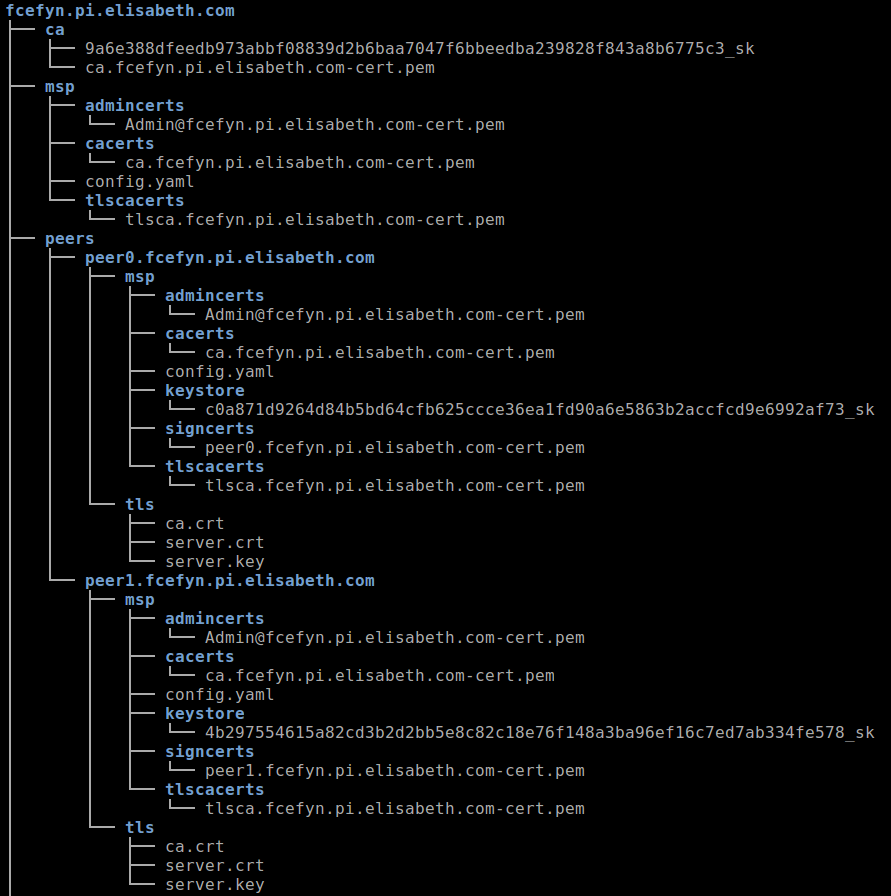
\includegraphics[width=0.8\linewidth]{Figures/Selection_191.png}}
        \caption{Directorios y archivos de la carpeta \textit{crypto-config}}
        \label{fig:crypto-config}
    \end{figure}
    \item \textbf{Generación del bloque de génesis y configuración del canal: }En el capítulo \ref{Chapter2} se explicó la arquitectura de un Blockchain: Información se almacena en bloques que contienen el \textit{hash} del bloque anterior y forman así una cadena de información. El primer bloque, llamado bloque de génesis, tiene la particularidad de almacenar solamente su propio \textit{hash}, ya que no tiene \textit{hash} de ningún bloque anterior que almacenar.
    
    En Hyperledger Fabric, el bloque de génesis cumple con un rol particular: Almacena la configuración del servicio que ordena transacciones y además información sobre las organizaciones y \textit{peers} que van a formar parte de la red. Un conjunto de organizaciones en este contexto se llama consorcio.

    Junto con el bloque de génesis se necesita la configuración del canal, que en Hyperledger Fabric describe el consorcio que va a tener acceso a un mismo \textit{ledger}.

    El bloque de génesis y la configuración del canal son llamados artefactos y son generados con la herramienta \textit{configtxgen}. Cómo \textit{cryptogen}, consume un archivo que contiene descripciones de los miembros de la red como del servicio de ordenamiento de transacciones. A continuación se van a describir las dos secciones más importantes del archivo de configuración:
    \inputminted[linenos, breaklines, bgcolor=mygray, firstline=97, lastline=105]{yaml}{Listings/configtx.yaml}
    En las líneas 97 a 105 se especifica el funcionamiento del servicio de ordenamiento de transacciones: Como tipo se eligió \textit{solo} (con las alternativas Raft y Kafka detalladas en la sección \ref{sec:ordering_service}) y se especificó un tiempo de espera de lote (\textit{BatchTimeout}) de dos segundos junto con un tamaño de lote (\textit{BatchSize}) de 512KB y un máximo de 99MB. Es decir, un bloque nuevo se genera cada dos segundos, sino se llegó antes al tamaño de lote definido.

    \inputminted[linenos, bgcolor=mygray, firstline=139, lastline=164]{yaml}{Listings/configtx.yaml}

    En las líneas 139 - 153 se define la configuración que se guarda en el bloque de génesis: Se compone por un consorcio, es decir, las tres organizaciones ya identificadas en el archivo crypto-config.yaml y la organización responsable de ordenar transacciones, aqui llamada OrdererOrg.
    
    En las líneas 154 - 163 se especifican las organizaciones que van a tener acceso al mismo canal.

    El bloque de génesis se genera con el siguiente comando:
    \begin{minted}[breaklines]{bash}
    $./configtxgen -profile OrgsOrdererGenesis -channelID sys-channel -outputBlock ./channel-artifacts/genesis.block
    \end{minted}
    Luego se crea la transacción de configuración del canal con
    \begin{minted}[breaklines]{bash}
    $./configtxgen -profile OrgsChannel -outputCreateChannelTx ./channel-artifacts/channel.tx -channelID pichannel
    \end{minted}
    Para que \textit{peers} pueden comunicarse entre organizaciones, al menos uno por organización necesita tener el estado de \textit{anchor peer}. Dicha configuración se realiza con los comandos siguientes: 
    \begin{minted}[breaklines]{bash}
    $./configtxgen -profile OrgsChannel -outputAnchorPeersUpdate ./channel-artifacts/famafMSPanchors.tx -channelID pichannel -asOrg famafMSP
    $./configtxgen -profile OrgsChannel -outputAnchorPeersUpdate ./channel-artifacts/fcefynMSPanchors.tx -channelID pichannel -asOrg fcefynMSP
    $./configtxgen -profile OrgsChannel -outputAnchorPeersUpdate ./channel-artifacts/fcqMSPanchors.tx -channelID pichannel -asOrg fcqMSP
    \end{minted}
    Se puede comprobar que en la carpeta channel-artifacts se encuentran los dos artefactos generados.
    \begin{figure}[H]
        \center{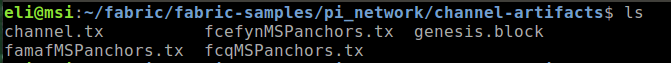
\includegraphics[width=1.0\linewidth]{Figures/Selection_199.png}}
        \caption{Artefactos generados por \textit{configtxgen}}
        \label{fig:configtxgen}
    \end{figure}

    \item \textbf{Iniciar los integrantes de la red con docker-compose: } Luego de la creación de los artefactos, el siguiente paso es iniciar todos los participantes de la red y compartirles los archivos generados. De esa forma pueden conocer su identidad y empezar a comunicarse con los demás participantes de la red. Para simular la cantidad de hosts requerida, se utilizaron las herramientas Docker y Docker Compose.
    
    La configuración de los \textit{peers}, autoridades de certificación y nodos de ordenamiento de transacciones se realizó en 3 archivos de docker-compose diferentes. El primero tiene el nombre \textit{peer-base.yaml} y define un \textit{peer} genérico con variables de entorno que aplican a todos los \textit{peers}, independiente de su organización. El segundo archivo, \textit{docker-compose-base.yaml}, describe todos los \textit{peers} que van a formar parte de la red con sus variables de entorno específicas. Un ejemplo provee la declaración del primer \textit{peer} de fcefyn:
    \inputminted[linenos, breakanywhere=true, breaklines, bgcolor=mygray, firstline=75, lastline=96]{yaml}{Listings/docker-compose-base.yaml}
    Líneas 78 y 79 muestran que el servicio extiende las propiedades descritas en \textit{peer-base.yaml}. En la sección \textit{environment} se declaran variables de entorno específicos del \textit{peer0} de la organización fcefyn y en la sección volúmenes se montan en primer lugar la transacción de configuración del canal y luego el material criptográfico generado con crypto-config.

    El tercer archivo, con el nombre \textit{docker-compose.yaml}, declara la topología completa de la red, extendiendo a \textit{docker-compose-base.yaml}. En una red llamada pi, se definen 3 autoridades de certificación, (una por organización), un total de 6 \textit{peers}, un \textit{orderer} y un contenedor auxiliar con el nombre cli.

    Para iniciar todos los contenedores, es necesario ejecutar el siguiente comando:
    \mint{bash}|$ docker-compose up -d|
    y luego se pueden ver los contenedores iniciados con el comando \mint{bash}|$ docker ps|
    \begin{figure}[H]
        \center{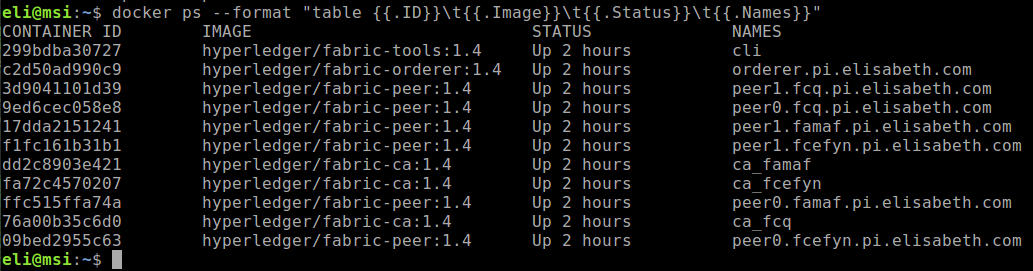
\includegraphics[width=1.0\linewidth]{Figures/Selection_193.png}}
        \caption{La red de Hyperledger Fabric desplegada con contenedores Docker}
        \label{fig:blockchain_network}
    \end{figure}
    En la figura \ref{fig:blockchain_network} se puede ver una captura en la cual figuran los contenedores previamente declarados. Se aplicó un filtro al comando para mejorar la visibilidad del resultado.
\item \textbf{Creación del canal y configuración de los peers: }Una vez que todos los contenedores se encuentran iniciados, es necesario crear el canal e indicar a todos los \textit{peers} que se unan al mismo. Para completar dicha tarea, existe el contenedor con el nombre cli, que permite ejecutar comandos en los \textit{peers} a través de una API.

Primero, se accede a la \textit{shell} del contenedor:
\begin{minted}{bash}
$ docker exec -it cli bash
\end{minted}
Luego, se ejecuta el siguiente comando para la creación del canal, haciendo uso del artefacto \textit{channel.tx} generado en el paso 2:
\begin{minted}[breaklines]{bash}
$ peer channel create -o orderer.pi.elisabeth.com:7050 -c pichannel -f ./channel-artifacts/channel.tx
\end{minted}
Para unir los demás \textit{peers} al canal, se ejecuta
\begin{minted}[breaklines]{bash}
$ peer channel join -b pichannel.block
\end{minted}
en cada \textit{peer}.

Con el fin de asegurar que el \textit{ledger} y el canal se crearon de forma exitosa, se puede inspeccionar el log de cualquier \textit{peer}:
\begin{figure}[H]
    \center{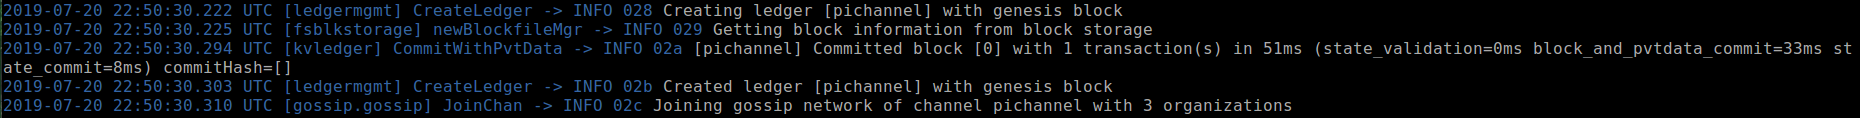
\includegraphics[width=1.0\linewidth]{Figures/Selection_197.png}}
    \caption{Mensajes del log de un \textit{peer} indicando que \textit{ledger} y canal se crearon de forma exitosa.}
    \label{fig:succesful_ledger}
\end{figure}

Por último, se aplican los artefactos que precisan los \textit{anchor \textit{peers}}. Aquí se ve el comando para la definición del \textit{anchor peer} de la organización fcq:
\begin{minted}[breaklines]{bash}
$ peer channel update -o orderer.pi.elisabeth.com:7050 -c pichannel -f ./channel-artifacts/fcqMSPanchors.tx
\end{minted}
En la figura \ref{fig:all_peers} se puede ver que todos los \textit{peers} se unieron al canal y que el peer0 de la organización fcq tiene conocimiento de todos los demás \textit{peers} de la red.
\begin{figure}[H]
    \center{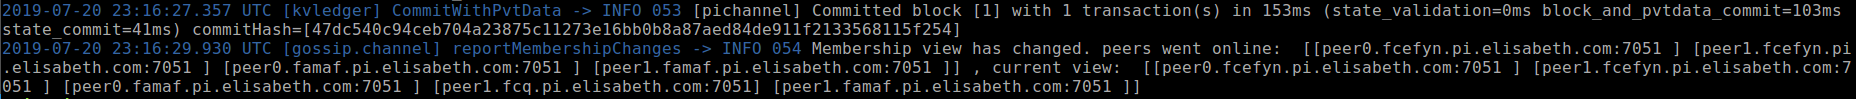
\includegraphics[width=1.0\linewidth]{Figures/Selection_198.png}}
    \caption{Mensajes del log de peer0.fcq.pi.elisabeth.com indicando todos los \textit{peers} conocidos.}
    \label{fig:all_peers}
\end{figure}
\item \textbf{Instalación y Uso del Chaincode: }Ya se logró configurar la red con todos sus participantes, pero todavía no es posible almacenar la información en el \textit{ledger}. Antes es necesario escribir e instalar el \textit{chaincode}.

El \textit{chaincode} en Hyperledger Fabric es el equivalente de los \textit{smart contracts} en otras implementaciones, como por ejemplo Ethereum. En el contexto de este proyecto, se escribieron tres chaincodes: \textit{addRegister} para agregar un acta al \textit{ledger}, \textit{queryRegister} para consultar por un acta y \textit{queryAllRectified} para obtener todas las actas rectificadas.

El \textit{chaincode} invoca la API presente en los \textit{peers}. A continuación se puede ver la función \textit{addRegister}: 
\begin{minted}[breaklines]{go}
    func (s *SmartContract) addRegister(APIstub shim.ChaincodeStubInterface, args []string) sc.Response {

	var buffer bytes.Buffer
	APIstub.PutState(args[0], []byte(args[1]))
	return shim.Success(buffer.Bytes())
}
\end{minted}

Luego de su redacción, es necesario instalar el \textit{chaincode} en todos los \textit{peers} que lo van a utilizar. Como en el caso de la configuración del canal, eso también se hace a través del contenedor cli. El comando para la instalación es el siguiente:
\begin{minted}[breaklines]{bash}
$ peer chaincode install -n picc -v 1.0 -p github.com/chaincode/
\end{minted}
Los mensajes correspondientes en los \textit{logs} del \textit{peer} confirman la instalación correcta, visibles en la figura \ref{fig:chaincode_logs}.
\begin{figure}[H]
    \center{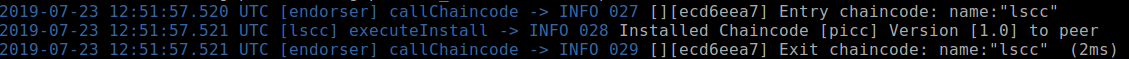
\includegraphics[width=1.0\linewidth]{Figures/Selection_203.png}}
    \caption{Mensajes del log de peer0.famaf.pi.elisabeth.com indicando la instalación correcta del \textit{chaincode}.}
    \label{fig:chaincode_logs}
\end{figure}
Luego es necesario instanciar al \textit{chaincode}, lo cual significa que se inicializa un contenedor Docker adicional en la misma red, en el cual el \textit{chaincode} se va a ejecutar. Mientras la instalación es necesaria en todos los \textit{peers}, la instanciación se requiere una sola vez.
\begin{minted}[breaklines]{bash}
$ docker exec cli peer chaincode instantiate -o orderer.pi.elisabeth.com:7050 -C pichannel -n picc -v 1.0 -c '{"Args":[]}' -P "OutOf (2, 'famafMSP.peer', 'fcefynMSP.peer', 'fcqMSP.peer')"
\end{minted}
El último argumento indica la política de aprobación: Se definió que dos \textit{peers} de diferentes organizaciones tienen que haber ejecutado el \textit{chaincode} y haber llegado al mismo resultado, caso contrario la operación no va a ser agregada al \textit{ledger}.

Por último, se verifica el funcionamiento correcto de la red invocando el \textit{chaincode} instalado. Éste tiene 3 funciones: \textit{addRegister} para agregar un acta, \textit{queryRegister} para consultar por un acta y \textit{queryAllRectified} para obtener todos los actas rectificadas.

Desde el contenedor cli, se ejecutó primero el comando siguiente:
\begin{minted}[breaklines]{bash}
$ peer chaincode invoke -o orderer.pi.elisabeth.com:7050 -C pichannel -n picc --peerAddresses peer0.famaf.pi.elisabeth.com:7051 --peerAddresses peer0.fcefyn.pi.elisabeth.com:7051 -c '{"Args":["addRegister", "UNC111", "{'UNC111':'testregister'}"]}'
\end{minted}
Para poder cumplir con la política de aprobación, la petición se envía a dos \textit{peers} de organizaciones diferentes. La información a escribir es un \textit{string} de prueba en formato JSON.
Luego se puede consultar por el acta ``UNC111'' con la función \textit{queryRegister}:
\begin{minted}[breaklines]{bash}
$ peer chaincode query -C pichannel -n picc -c '{"Args":["queryRegister","UNC111"]}'
\end{minted}
con el resultado visible en la figura \ref{fig:query_reg_call}
\begin{figure}[H]
    \center{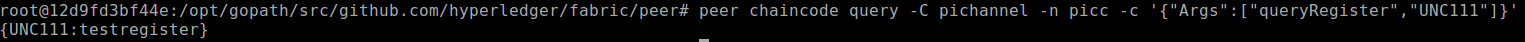
\includegraphics[width=1.0\linewidth]{Figures/Selection_208.png}}
    \caption{Respuesta de la llamada a la función \textit{queryRegister}}
    \label{fig:query_reg_call}
\end{figure}
\end{enumerate}
Con los pasos descritos quedan concluidas la configuración y las pruebas de la red de Hyperledger Fabric en un ambiente local.
\subsection{Automatización con un bash script}
Dada la numerosa cantidad de pasos a ejecutar, la importancia de escribir los parámetros y los variables de entorno correctamente y la necesidad de ejecutar pruebas con una red nueva, se automatizó el proceso descrito en la sección anterior mediante un \textit
{script} en el lenguaje \textit{bash}. Al ejecutarlo, 
\begin{itemize}
    \item Se eliminan todos los contenedores, volúmenes, redes y material criptográfico que pueden existir de una ejecución anterior.
    \item Se generan nuevamente los artefactos.
    \item Se inician todos los contenedores especificados en el archivo docker-compose.yaml.
    \item Se configuran canal y \textit{anchor peers}.
    \item Se instala el \textit{chaincode} en todos los \textit{peers} y se instancia.
\end{itemize}
Luego de la ejecución, es posible invocar al \textit{chaincode} directamente. El \textit{bash script} posibilita el avance rápido con los otros elementos del proyecto, ya que en caso de ocurrir errores, simplemente se genera una red con material criptográfico nuevo y sin datos previamente almacenados.

\subsection{Implementación de la Aplicación con API}
Al desarrollar la aplicación en Javascript, se partió con las funciones definidas en el ejemplo de Hyperledger Fabric disponible en \href{https://github.com/hyperledger/fabric-samples/tree/release/fabcar}{https://github.com/hyperledger/fabric-samples/tree/release/fabcar}. Luego de descargar los archivos \textit{enrollAdmin.js}, \textit{registerUser.js}, \textit{query.js} e \textit{invoke.js} junto con el respectivo \textit{package.json}, se ejecutó el comando
\begin{minted}{bash}
$ npm install
\end{minted}
Para iniciar el ambiente e instalar todos los módulos requeridos de node.js. Con el fin de que la aplicación se reinicie automáticamente cuando ocurran cambios de código, se instaló nodemon:
\begin{minted}{bash}
$ npm install nodemon --save
\end{minted}

La aplicación necesita información sobre la topología de la red a la cual conectarse. Se define a través del archivo \textit{connection.json}, que indica canales, organizaciones, \textit{peers} y autoridades de certificación. A continuación, se ve una parte del archivo en cuestión:
\inputminted[linenos, breakanywhere=true, breaklines, bgcolor=mygray, firstline=16, lastline=40]{json}{Listings/connection.json}

Las funciones separadas que se descargaron son útiles para comprobar el funcionamiento correcto del SDK, pero no es un formato conveniente para que sean invocadas desde una aplicación web. Por ende, los pasos a seguir consisten en:
\begin{enumerate}
    \item Implementar una API con el \textit{framework} Express.
    \item Embeber las funciones descargadas para que puedan acceder al Blockchain cuando se llame la API.
    \item Desarrollar y agregar las demás funciones necesarias para cumplir con los requerimientos definidos en el capítulo \ref{Chapter4}.
\end{enumerate}

\begin{enumerate}
    \item \textbf{Implementación de una API REST con el framework Express}\newline
    Se empezó con el código de un servidor web que responde a una sola consulta:
    \inputminted[linenos, breakanywhere=true, breaklines, bgcolor=mygray]{js}{Listings/example.js}
    Luego se usó el \textit{software} Postman para comprobar el correcto funcionamiento del programa.
    \begin{figure}[H]
        \center{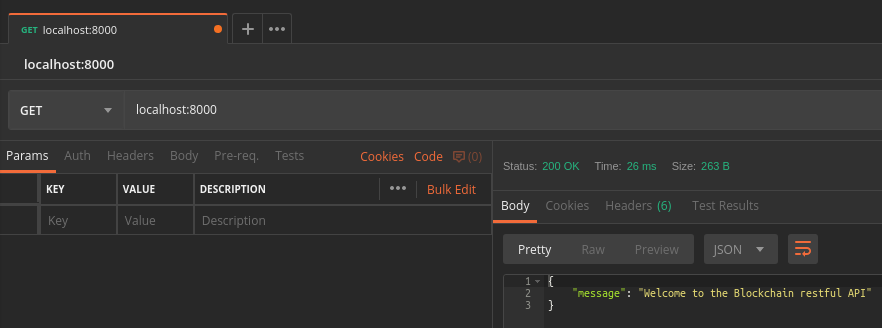
\includegraphics[width=1.0\linewidth]{Figures/Selection_213.png}}
        \caption{Prueba de la función GET con Postman}
        \label{fig:postman_first}
    \end{figure}
    En la figura \ref{fig:postman_first} se puede observar que la aplicación está funcionando correctamente, ya que devuelve el mensaje \textit{``Welcome to the Blockchain restful API''}.
    \item \textbf{Ampliación de la API para registrar usuarios}\newline
    En primer lugar, es necesario inscribir al administrador y luego registrar al usuario que va a invocar al \textit{chaincode}. En el contexto del proyecto integrador, se va a crear un solo usuario con el nombre \textit{user1} para la organización fcefyn, sin embargo es posible ampliar la cantidad de usuarios fácilmente con la ayuda de la función ya escrita.
    Como el foco de la aplicación es cargar actas y validar sus entradas, la API controla de forma automática que \textit{admin} y \textit{user1} estén registrados:
    \begin{minted}[linenos, breakanywhere=true, breaklines, bgcolor=mygray]{js}
    app.listen(3000, () => {
        console.log("Server running on port 3000");
        enroll_admin.enrollAdmin().then(
            success => {
                setTimeout(() => register_user.registerUser(), 1000)
            })
        });
    \end{minted}
\end{enumerate}
\subsubsection{Desarrollo de la función \textit{add\_register}}
La primera función a desarrollar agrega actas al Blockchain, ya que se necesitan datos presentes en el \textit{ledger} para poder programar funciones futuras que, por ejemplo, validen dichos datos.

Un acta en el contexto de este proyecto tiene formato JSON. En una cabecera se describen los atributos del acta en sí y una cantidad arbitraria de renglones especifica los datos de los alumnos. Un ejemplo con dos renglones sigue a continuación:
\begin{minted}[linenos, breakanywhere=true, breaklines, bgcolor=mygray]{json}
{
    "UNC201200017":{
    "Acta Nr":"201200017",
    "Año academico":"2016",
    "Actividad":"(1001) Análisis matemático 1a",
    "Fecha Examen":"05/10/2016",
    "Turno": "Octubre 2016",
    "Ubicación": "Sede Av Santa Fe",
    "Mesa": "A",
    "Llamado": "Llamado del Turno Octubre 2016"
    },

    "Renglones":{
        "1":{
        "Appellido y Nombre":"Acevedo Mauricio German",
        "Identificacón:":"DNI 4260181",
        "Instancia": "Regular",
        "Fecha": "05/10/2017",
        "Nota": 2,
        "Letras": "dos",
        "Resultado": "reprobado"},

        "2":{
        "Appellido y Nombre":"Alaniz Roxana Aide",
        "Identificacón:":"DNI 9609175",
        "Instancia": "Regular",
        "Fecha": "05/10/2017",
        "Nota": 8,
        "Letras": "ocho",
        "Resultado": "aprobado"}
    }
}
\end{minted}
La figura \ref{fig:actividad_add_register} muestra la lógica de la función implementada: Se aplican funciones \textit{hash} al id, a la cabecera y a cada uno de los renglones y luego se genera un JSON nuevo con dicha información que tiene el siguiente aspecto: 
\begin{minted}[linenos, breakanywhere=true, breaklines, bgcolor=mygray]{json}
{
  "id": "d7ce098a17e4bb0cc49041382beb8577",
  "header": "8bb106442e641e7af465bd40cf54375e",
  "validity": "valid",
  "creator": "user1",
  "lines": 
   { "1": "81116f6d2bdf1728e17d0258d54a74e9",
     "2": "b1af6ddd90993bdd9763e45e280cbb6b" }
}
\end{minted}
\begin{figure}
    \center{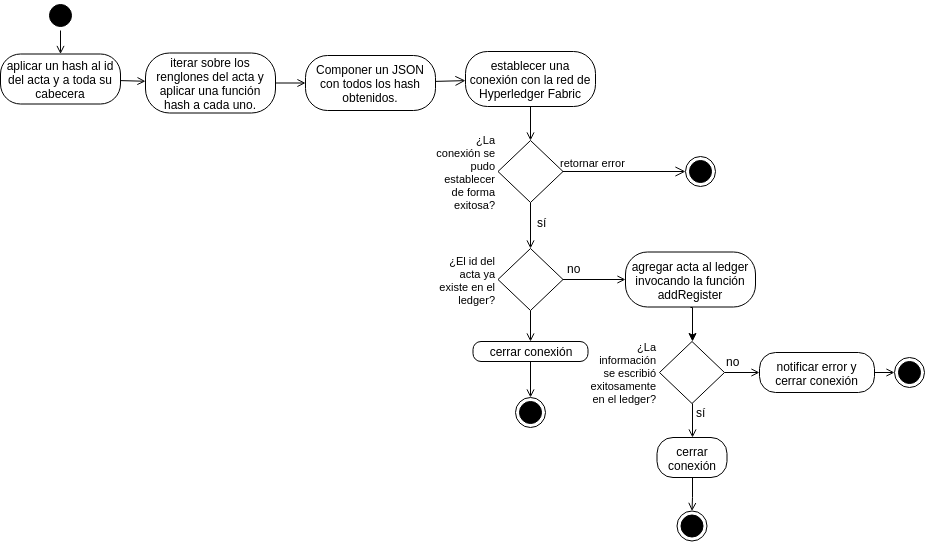
\includegraphics[width=0.8\linewidth]{Figures/actividad1.png}}
    \caption{Diagrama de actividad de la función add\_register}
    \label{fig:actividad_add_register}
\end{figure}

Luego, se establece una conexión con la red de Hyperledger Fabric y se invoca el \textit{chaincode} \textit{queryRegister} con el id del acta como parámetro. Dicha consulta se hace para verificar que el acta todavía no fue agregada al Blockchain. Si se encuentra una entrada con el mismo id, la conexión se cierra y la API devuelve un mensaje de error especificando que el acta ya existe. Caso contrario se invoca a la función \textit{addRegister} con los parámetros ``UNC201200017'' y el JSON con los \textit{hash}. Si la operación de escritura fue exitosa, la API devuelve el mensaje ``El acta se subió exitosamente'' como se ve en la figura \ref{fig:add_register_api}.

\begin{figure}[H]
    \center{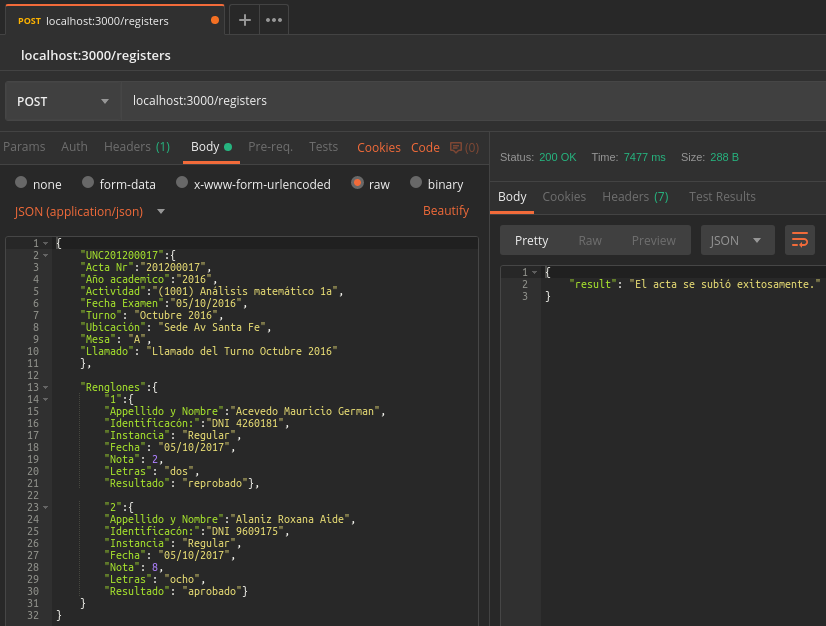
\includegraphics[width=0.7\linewidth]{Figures/Selection_220.png}}
    \caption{Subida exitosa de un acta a través de la API.}
    \label{fig:add_register_api}
\end{figure}

\subsubsection{Desarrollo de la función \textit{query}}
La función \textit{query} está pensada para poder comprobar el funcionamiento correcto del sistema, no para el uso del personal administrativo. Su objetivo es recuperar el acta como se agregó al Blockchain haciendo uso del \textit{chaincode} \textit{queryRegister}.
En la figura \ref{fig:query_register_api} es posible ver la llamada al Blockchain junto a su respuesta constando de la información previamente subida.
\begin{figure}[H]
    \center{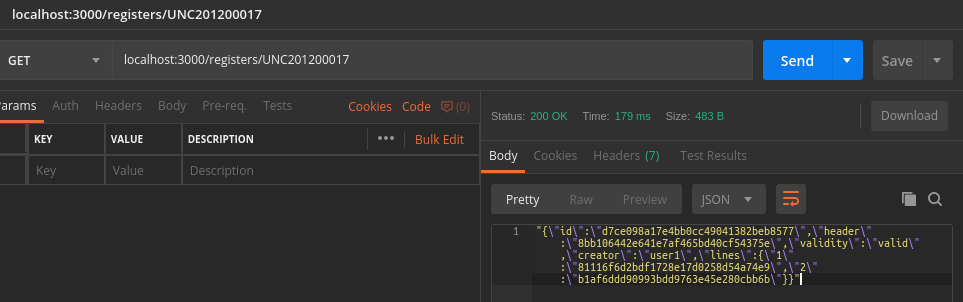
\includegraphics[width=1.0\linewidth]{Figures/Selection_221.png}}
    \caption{Consulta de un acta por Postman.}
    \label{fig:query_register_api}
\end{figure}
En el caso de consultar por un id inexistente, la API responde con el mensaje ``Acta no encontrada.''

\subsubsection{Desarrollo de la función \textit{check\_validity}}
Luego de haber subido un acta al Blockchain, ya es posible implementar la función que verifique la validez de una nota. La secuencia de pasos a implementar se puede ver en la figura  \ref{fig:validate_grade}.
\begin{figure}[H]
    \center{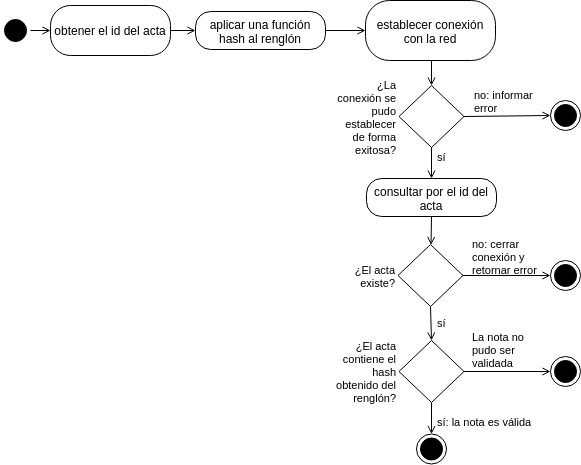
\includegraphics[width=0.6\linewidth]{Figures/actividad3.png}}
    \caption{Diagrama de actividad para el caso de validación de una nota.}
    \label{fig:validate_grade}
\end{figure}
En primer lugar, se envía un objeto JSON a la API que contiene el id del acta junto al renglón que se quiere validar. La API aplica la misma función \textit{hash} al renglón que fue aplicada en el momento de subir el acta. Luego se establece una conexión con la red y se consulta por el acta en cuestión. Si éste existe, se busca el \textit{hash} recientemente calculado entre los renglones del acta almacenada en el Blockchain. Si existe una coincidencia, la nota es válida, en caso contrario, la nota se declara inválida. En la figura \ref{fig:validate_grade_api}, se ve el caso de la validación exitosa de la nota de un alumno ficticio con el nombre Mauricio German Acevedo.
\begin{figure}[H]
    \center{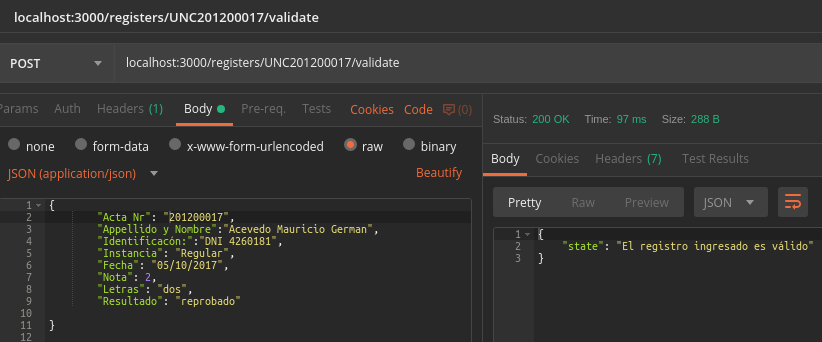
\includegraphics[width=0.8\linewidth]{Figures/Selection_222.png}}
    \caption{Validación exitosa de una nota.}
    \label{fig:validate_grade_api}
\end{figure}
\subsubsection{Desarrollo de la función \textit{verify\_history}}
La función que verifica la validez de una historia académica funciona de forma muy parecida a la que verifica la validez de una sola nota: La API itera sobre los renglones, aplica la función \textit{hash} a cada uno y busca una coincidencia con los \textit{hash} presentes en las actas obtenidos. La figura \ref{fig:validate_history_api} muestra la consulta realizada junto con el resultado que la API entrega: Como hasta el momento solo se agregó un acta al Blockchain, tres de los cuatro actas no fueron encontradas. La historia académica completa solamente puede ser considerada válida si la totalidad de respuestas indica notas válidas.
\begin{figure}
    \center{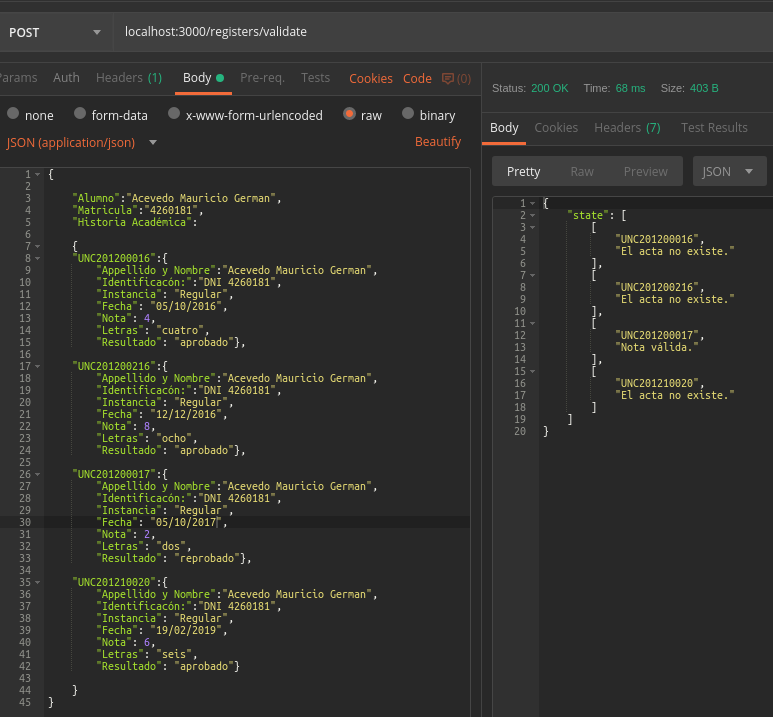
\includegraphics[width=0.9\linewidth]{Figures/Selection_223.png}}
    \caption{Validación de una historia académica.}
    \label{fig:validate_history_api}
\end{figure}
\subsubsection{Desarrollo de la función \textit{add\_revoked}}
Ahora que ya es posible subir actas y validar notas, falta la implementación del requerimiento que permite revocar un acta. El diagrama de actividad para dicha función se puede ver en la figura \ref{fig:activity_revoke}. Para demostrar el flujo con un ejemplo, se va a asumir que ocurrió un error al reprobar el alumno Mauricio German Acevedo en el acta 201200017 y que es necesario corregir la nota por un cuatro. La corrección afectaría a un solo renglón de un total de 2 renglones del acta.
Un objeto JSON muestra la información que se envía a la API para invocar las funciones correspondientes.
\begin{figure}
    \center{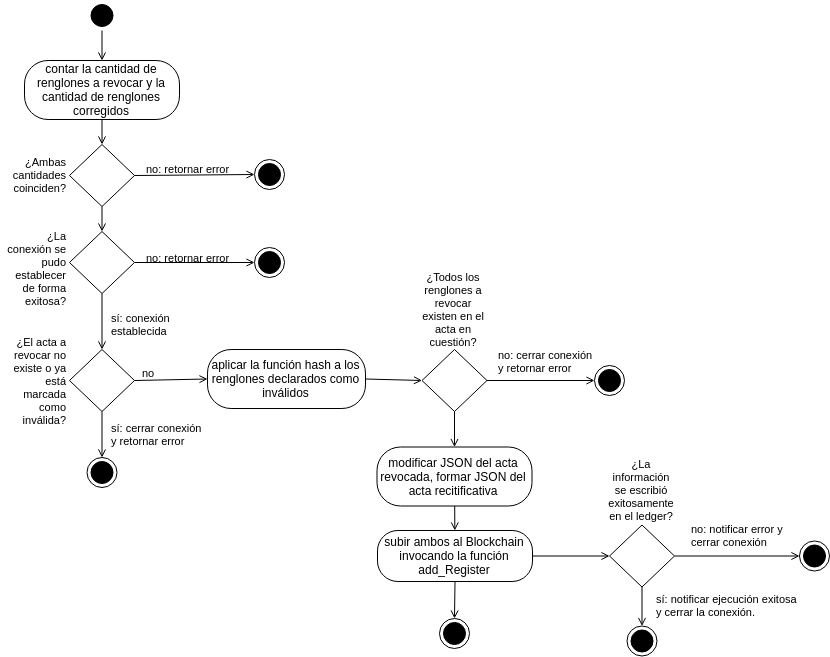
\includegraphics[width=0.7\linewidth]{Figures/actividad4.png}}
    \caption{Diagrama de actividad para revocar un acta.}
    \label{fig:activity_revoke}
\end{figure}
\begin{minted}[linenos, breakanywhere=true, breaklines, bgcolor=mygray]{json}
{    "Acta Nr":"201200017",

    "revocar":{

        "1":{
        "Appellido y Nombre":"Acevedo Mauricio German",
        "Identificacón:":"DNI 4260181",
        "Instancia": "Regular",
        "Fecha": "05/10/2017",
        "Nota": 2,
        "Letras": "dos",
        "Resultado": "reprobado"}
    },
    "corregido":{
         "1":{
        "Appellido y Nombre":"Acevedo Mauricio German",
        "Identificacón:":"DNI 4260181",
        "Instancia": "Regular",
        "Fecha": "05/10/2017",
        "Nota": 4,
        "Letras": "cuatro",
        "Resultado": "aprobado"}
	}
}
\end{minted}
Los pasos que efecúa la API son los siguientes:
\begin{enumerate}
    \item Se verifica que la cantidad de renglones a revocar coincida con la cantidad de renglones corregidos, caso contrario quedarían renglones revocados sin corregir o se corregirían renglones que no fueron revocados.
    \item Después de que la API pudo establecer una conexión con la red, verifica que el acta a revocar existe y es válida. Si no sería posible crear un acta rectificativa para un acta inexistente o una que ya tiene acta rectificativa, en cuyo caso existirían dos actas rectificativas para una sola acta revocada. En el contexto del proyecto presente, solamente es posible corregir un acta una sola vez.
    \item Si es posible revocar el acta, se aplica la función \textit{hash} a todos los renglones: los que se van a revocar y los que van a corregir los revocados. Se verifica que los renglones a revocar realmente existen en el acta en cuestión, ya que si no fuera el caso, se estaría revocando información inexistente.
    \item Si todas las verificaciones anteriores resultaran exitosas, se genera el acta nueva reemplazando los \textit{hash} de los renglones revocados por los \textit{hash} de los renglones corregidos. El id de cualquier acta rectificativa inicia con las letras RECT, para poder distinguirlo de actas que no fueron corregidas.
    
    Por otro lado, se modifica el acta revocada, cambiando el valor de la clave ``validity'' por ``invalid'' y agregando una clave ``revoked lines'' que lleva como valor los \textit{hash} de las líneas que fueron revocadas. Es necesario recordar que en el caso de una consulta al \textit{ledger} con la función \textit{query}, el \textit{peer} consulta al \textit{world state}, que siempre indica el valor más actual de un objeto almacenado. Una vez que se revocó el acta 201200017, una consulta siempre va recuperar el acta con estado inválido. Si se consulta por el historial de la misma acta, va a haber dos entradas: el original y luego el revocado.
    \item Por último, se actualiza el acta revocada y se agrega el acta rectificativa al Blockchain.
\end{enumerate}
\begin{figure}[H]
    \center{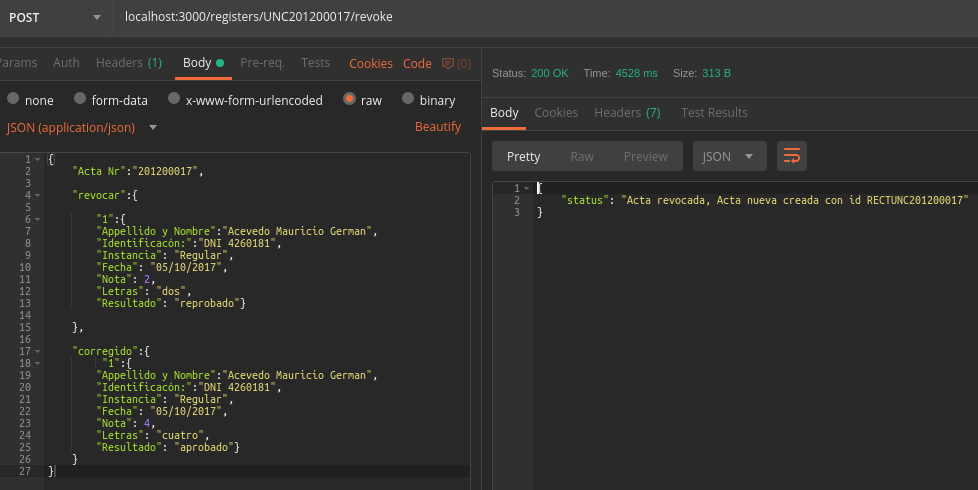
\includegraphics[width=0.9\linewidth]{Figures/Selection_224.png}}
    \caption{Creación de un acta rectificativa.}
    \label{fig:revoke_api}
\end{figure}
En la figura \ref{fig:revoke_api} se puede ver la respuesta de la API en el caso de una corrección exitosa. Se indica el id del acta rectificativa. Si ahora se hace una consulta a \textit{localhost:3000/registers/UNC201200017} (figura \ref{fig:invalid_register}), se puede ver que el estado es inválido y se agregó la clave ``revoked\_lines'', de la cual se habló anteriormente.
\begin{figure}
    \center{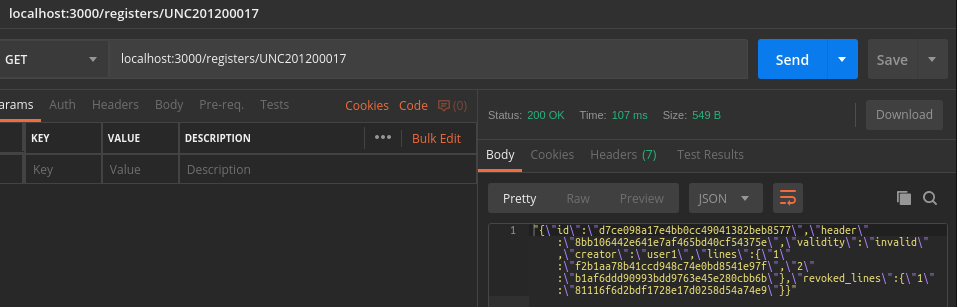
\includegraphics[width=0.9\linewidth]{Figures/Selection_225.png}}
    \caption{Consulta de un acta inválida.}
    \label{fig:invalid_register}
\end{figure}

Como última prueba es necesario corroborar que las actas revocadas no se tienen en cuenta a la hora de validar una historia académica: En la figura \ref{fig:history_with_revoked} se puede observar la consulta por la validez de la historia académica de Mauricio German Acevedo con el aplazo corregido en el acta 201200017. La nota aparece válida, lo cual indica que el sistema está teniendo en cuenta de manera correcta las actas revocadas y sus actas rectificativas.

\begin{figure}[H]
    \center{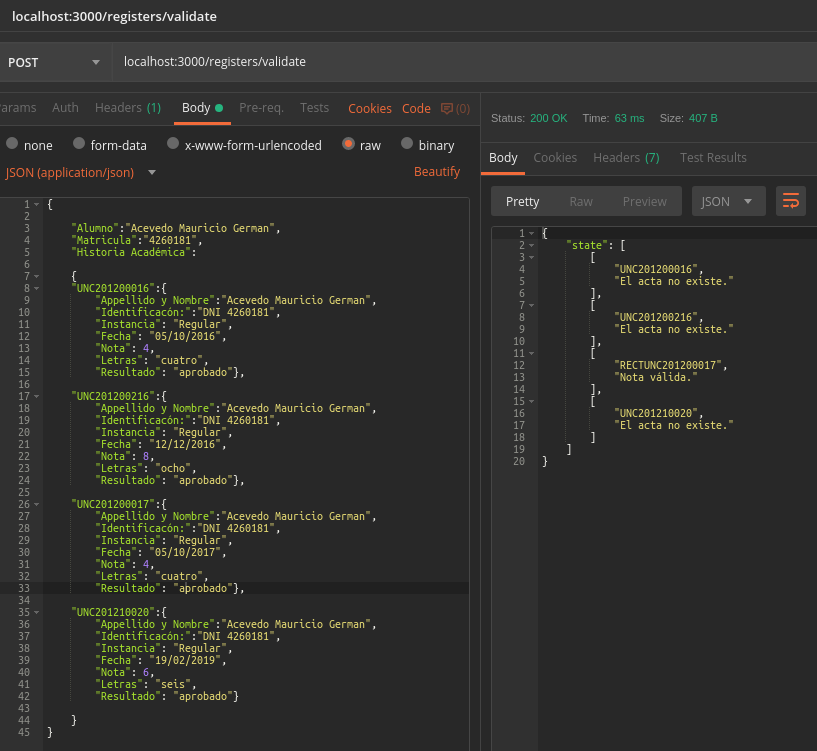
\includegraphics[width=0.9\linewidth]{Figures/Selection_226.png}}
    \caption{Validación de una historia académica involucrando un acta rectificativa.}
    \label{fig:history_with_revoked}
\end{figure}
\subsubsection{Desarrollo de la función \textit{query\_rectified}}
La función es implementada de la misma forma que \textit{query}, pero invoca al \textit{chaincode} \textit{queryAllRectified}, el cual tiene la particularidad de filtrar todas las actas con el prefijo ``RECT''. En la captura \ref{fig:all_rectified}, aparece solo un acta, porque en el momento de la prueba no se habían cargado y revocado más actas, sin embargo siempre figurará la cantidad correspondiente a las actas rectificadas.
\begin{figure}
    \center{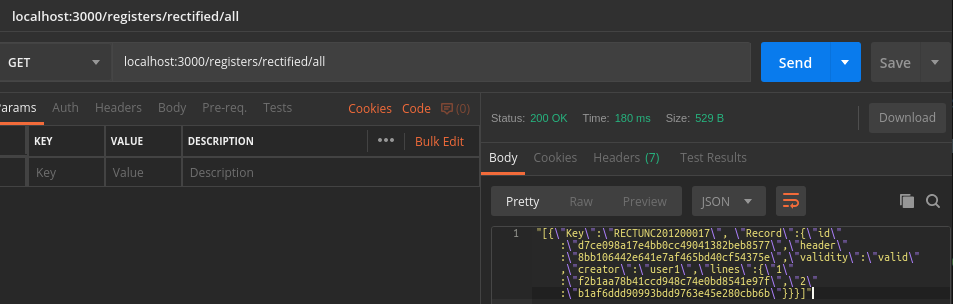
\includegraphics[width=0.9\linewidth]{Figures/Selection_227.png}}
    \caption{Consulta por todas las actas rectificativas.}
    \label{fig:all_rectified}
\end{figure}
\subsection{Implementación del Frontend con Angular e Ionic}
Luego de las instalaciones de Angular e Ionic descritas en la sección \ref{instalation_frontend} se procedió a eliminar el contenido por defecto que lleva la aplicación de prueba. Luego, se siguieron los siguientes pasos de desarrollo:
\begin{itemize}
    \item Con la ayuda del comando
    \begin{minted}{bash}
$ ionic generate page <pagename>
    \end{minted}
se generaron en total 6 páginas, una por cada caso de uso.
    \item El objetivo de la página principal, \textit{home}, es proveer una visión general de las funcionalidades de la implementación. Para eso se utilizó la estructura \textit{ion-grid}, donde cada cuadrícula presenta uno de los casos de uso descritos. Se agregaron imágenes descriptivas para facilitar la navegación por la página. En la figura \ref{fig:home_page}, se puede ver dicha implementación.
    \begin{figure}[H]
        \center{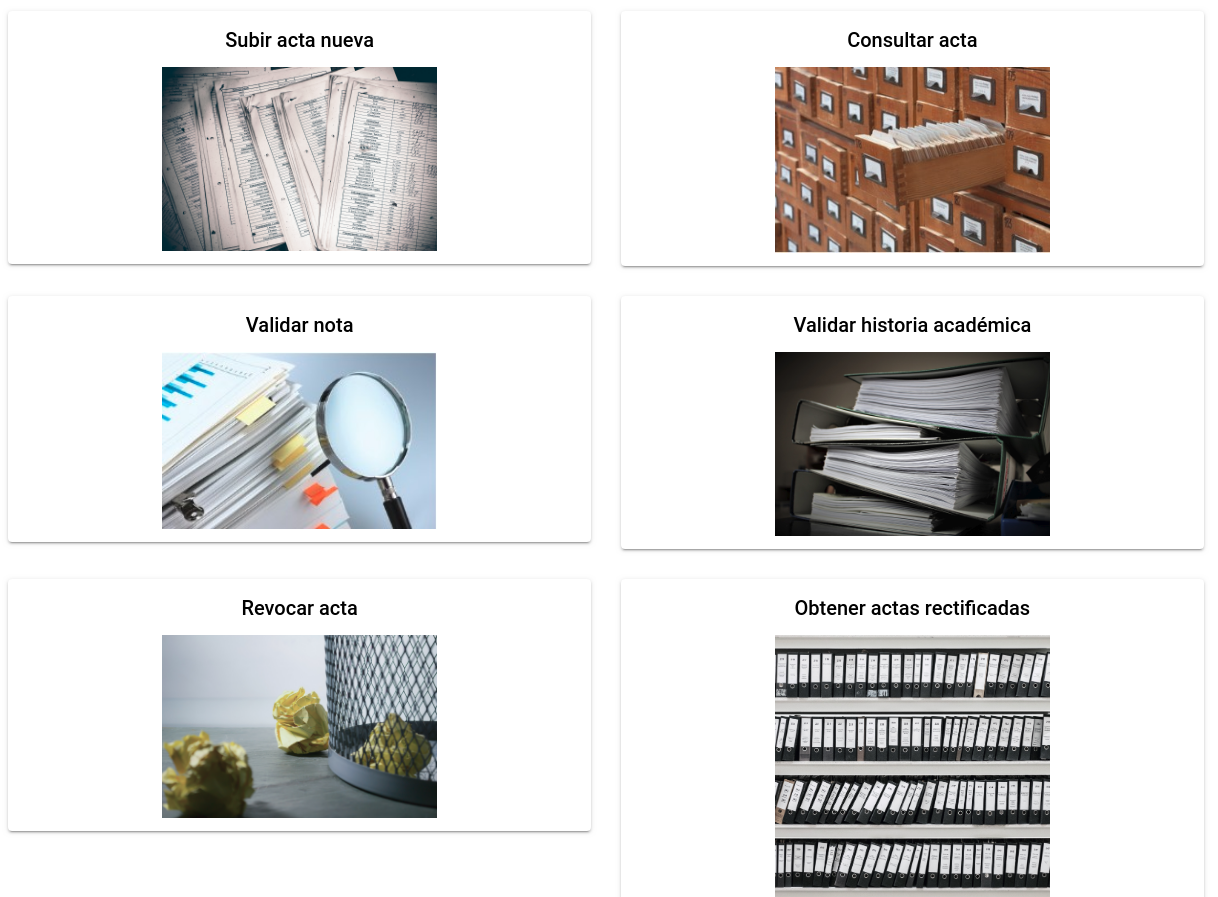
\includegraphics[width=0.7\linewidth]{Figures/Selection_228.png}}
        \caption{\textit{ion-grid} con los 6 casos de uso.}
        \label{fig:home_page}
    \end{figure}
    \item Al hacer clic en cada una de las cuadrículas, el usuario navega hacia la página correspondiente al caso de uso elegido. Ahí es presentado con un campo para una entrada de usuario, implementada mediante el componente \textit{ion-input}. Como en la mayoría de los casos la entrada del usuario tiene que tener formato JSON para ser enviada a la API, se verifica que los datos aportados realmente tengan dicho formato. En caso contrario, indica un error mediante el componente \textit{ion-toast} y la API no es invocada. Dicho caso se puede ver en la figura \ref{fig:json_toast}
    \begin{figure}[H]
        \center{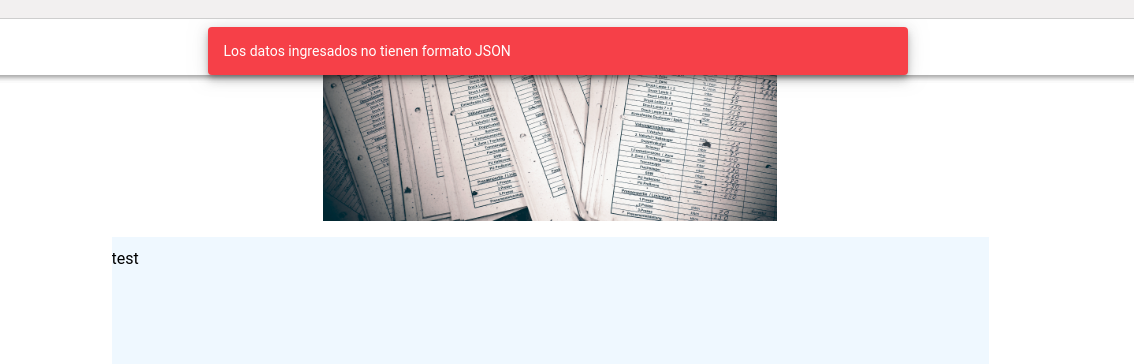
\includegraphics[width=0.8\linewidth]{Figures/Selection_229.png}}
        \caption{Un \textit{ion-toast} que indica que la entrada de usuario no se encuentra en formato JSON.}
        \label{fig:json_toast}
    \end{figure}
    \item Para notificar al usuario si los datos ingresados se escribieron exitosamente en el Blockchain, se empleó el componente \textit{ion-alert}. Dicho elemento abre una pequeña ventana que indica el éxito o fracaso de una operación y provee un mensaje de error si es necesario. En la figura \ref{fig:ion_alert} se muestran dos posibles alertas: en el primer caso, un acta se agregó exitosamente al Blockchain. Al querer subir la misma acta nuevamente, se produce el error visible a la derecha: si bien se pudo acceder al Blockchain, no fue posible escribir en él ya que el acta existía anteriormente.
    \begin{figure}[H]
        \center{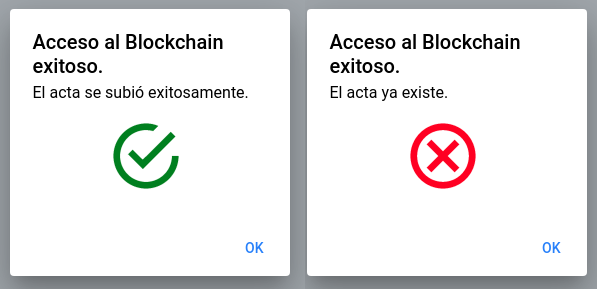
\includegraphics[width=0.8\linewidth]{Figures/Selection_232.png}}
        \caption{Alertas de notificación sobre el éxito o fracaso de una operación.}
        \label{fig:ion_alert}
    \end{figure}
    \item Para que los usuarios que desconocen el sistema puedan utilizar el mismo, se generó una página adicional de ayuda, que provee instrucciones y ejemplos.
    \item Por último, se agregó la funcionalidad de traducción de la página web con el módulo @ngx-translate/core. En la parte superior se encuentran la bandera española junto a la bandera estado-unidense. Seleccionar la bandera a elección modifica el idioma en el que aparece la página.
\end{itemize}

%\section{Implementación en un clúster Kubernetes}
%\subsection{Migración de Hyperledger Fabric}
%\subsection{Migración de la Aplicación}
%\subsection{Migración del Frontend}

